\newpage
\begin{center}
  \textbf{\large АННОТАЦИЯ}
\end{center}

Один из способов косвенного обнаружения темной материи --- детектирование сигнала нейтринными обсерваториями потоков нейтрино, образующихся в результате аннигиляции темной материи, которая захватывается накапливается  в гравитационном поле небесных обектов, таких как Солнце или Земля. На данный момент этот сигнал не обнаружен, накладывает ограничения на сечение взаимодействия частицы темной материи и протона. В данной работе мы получим такие ограничения для неупругой темной материи состоящей из основного и возбужденоного состояния, для которой ограничения на сечения ослабленны по сравнению с упругой темной материей. Мы учтем процесс термализации и численно решим уравниние эволюции, чтобы вычислить аннигиляционные потоки, поскольку неупругая темная материя при большой разнице масс основного и возбужденного состояния не успевает термализоваться, что приводит к еще большему ослаблению ограничений на сечение.

\onehalfspacing
\setcounter{page}{2}

\newpage
\renewcommand{\contentsname}{\centerline{\large СОДЕРЖАНИЕ}}
\tableofcontents

\newpage
\begin{center}
  \textbf{\large ВВЕДЕНИЕ}
\end{center}
\addcontentsline{toc}{chapter}{ВВЕДЕНИЕ}


Одна из основных проблем современной космологии --- это проблема темной материи.  Темная материя --- это часть нерелятивисткой материи, находящейся во вселенной, которая не наблюдается напрямую, однако участвует в расширении вселенной, образовании структур. 


Наблюдения за астрономическими объектами и исследование анизотропии реликтового излучения позволяет найти основные параметры космологических моделей , такие как доля материи (нерелятивисткого вещества) и барионной материи. Для современных космологических моделей доля вещества в настоящий момент составляет $\Omega_M = 0.2-0.3$, при этом барионная материя составляет $0.03-0.05$ \cite{Cao_2023}. Большая чать вещества во вселенной остается не объясненной наблюдаемой материей.

На наличие темной материи также указывают наблюдения скоростей звезд внутри галактик. Исследование скоростей звезд внутри галактик позволяет найти распределение массы и плотность материи \cite{Radial_velocity_measurements}, \cite{Angular_Velocity}. Отношение измеренной таким образом массы и массы наблюдаемого светимого вещества оказывается значительно больше единицы. Аналогичные исследования позволяют найти локальную плотность темной матери в солнечной системе. Эта плотность равна $\rho_{DM} = 0.2 - 0.4, GeV \cdot cm^{-3}$ \cite{palau2022oblateness}. В данной работе мы будем использовать значение  $\rho_{DM} = 0.4, GeV \cdot  cm^{-3}$.


Возможны разные способы объянить темную материю. Так, в качестве темной материи могут являються массивные астрономические компактные объекты (первичные черные дыры с массой порядка $10-100M_{\odot}$). Такие объекты могут быть обнаружены с помощью измерения светимости и гравитационного линзирования, и сегодняшний день наблюдения дают ограничения на их долю в массе нерелятивисткого вещества в районе $0.15-0.3$ \cite{Zumalac_rregui_2018}, \cite{Blaineau_2022}.
Также существуют различные модификации теории гравитации которые могут объясняснить кривые вращения или вклад материи в метрики без включения в модель новых частиц \cite{1984ApJ...286....7B}.


Наиболее распространенные же модели ТМ предполагают наличие новых частиц вне 
стандартной модели (СМ), которые находятся в активном поиске. В качестве кандитатов рассмитривают, например, майорановские стерильные нейтрино в $keV$ном диапазоне масс \cite{Boyarsky_2019}, наличие которых может указать регистрация двойного безнейтринный $\beta$-распада или спектральных линии фотонов, соответствующие их распаду. Также, темной материей могут быть аксионы, призванные решить проблему сильных CP нарушений, которые могут осциллировать в фотоны в сильных э-м. полях \cite{adams2023axion}. Частицы ТМ появляются и в суперсимметричных расширениях СМ \cite{berezinsky1996dark}, так как из-зи сохранения R-четности, легчайшая частица-суперпартнер становится стабильной и может быть основой для WIMPов, о которых будет идти речь далее.

WIMP, массивная слабовзаимодействующая частица, --- это частица темной материи в широком диапазоне масс ($MeV-TeV$). Предполагается, что такие частицы находились в термальном равновесии с остальной материей на ранних этапах эволюции вселенной. Затем, при расширении вселенной, когда темп аниигиляции становится меньше, чем темп расширения (постоянная хаббла на соответствующий момент времени), эти частицы замораживаются будучи нерелятивисткими\cite{Kolb:1990vq}. Температура фризаута определяется соотножением 
\begin{equation}
	x_f = \cfrac{m_{\chi} }{T_f} = \ln {\left(\cfrac{0.038 g_{\chi} M_{pl} m_{\chi}  \average{\sigma_{ann} v}}
		{\sqrt{g_* x_f}}\right)}
\end{equation}
где $g_{\chi}$ и $g_*$ --- стемени свободы ТМ и релятивисткого вещества, $M_{pl}$ --- масса планка, $\sigma_{ann} v = \sigma_0$ --- сечение аннигиляции. И доля темной материи, состоящий из этих частиц, равна 
\begin{equation}
	\Omega{\chi} = \cfrac{\sn{1.9}{-27} x_f}{\sqrt{g_*} \sigma_0} \frac{cm^3}{s}
\end{equation}
При разумных параметрах ($x_f \approx 20, g_* \approx 80$), для объяснения сегогдняшней плотности темной материи механизмом фризаута необходимо, чтобы $\sigma_0 \approx 10^{26} cm^3s^{-1}$, порядку величины близко к слабым взаимодействиям.

WIMPы, находящиеся в гало, могут быть обнаружены прямыми методами в низкофоновых экспериментах. Такой способ детектирования основан на детектирования отдачи при взаимодействии частиц ТМ, находящихся в гало, с ядром \cite{Schumann_2019}. Наиболее известные эксперименты --- DAMA/LIBRA, COSINE-100, XENON100, XENON1T, CDMS, исользующие в качестве мишени NaI, Xe, Ge. На данный момент эти эксперименты на обнаружили значительного превышения сигнала над фоном, кроме DAMA/LIBRA, регистрирующий сигнал годовых модуляций, подтверждающий конепцию WIMPов \cite{Bernabei_2018}, однако, эксперимент COSINE-100, имеющий ту же мишень (NaI)  не подтвердил результаты \cite{Adhikari_2022}.

МЫ будем рассматривать косвенный метод обнаружения ТМ, основанный на детектировании аннигиляционных потоков частиц темной материи, захваченной небесными объектами. Частицы темной материи, взаимодействуя с веществом, сосредоточенном в астрономических объектах, передают им часть кинетической энергии. Это приводит к захвату в гравитационном потенциале небесного тела. В резальтате ТМ накапливается, что приводит к значительному усилению темпа аннигиляции. Таким образом создаются потоки нейтрино, которые возможно зарегистрировать в нейтринных обсерваториях  IceCube \cite{Aartsen_2017}, SuperKamiokande \cite{kamiokandecollaboration2015search}, ANTARES \cite{ADRIANMARTINEZ201669}. Для захвата частиц ТМ рассматривается Солнце \cite{1985ApJ...296..679P}, Землю \cite{1987ApJ...321..571G}, Юпитер \cite{10.1103/physrevd.106.115037} (для более легких WIMPов, так как температурное испарение ТМ на Юпитере значительно ниже). Отсутствие нейтринного сигнала дает ограничение ограничивает сечение взаимодействия с протоном $\sigma_{\chi p}$.

\begin{figure}[htb]
	\begin{center}
		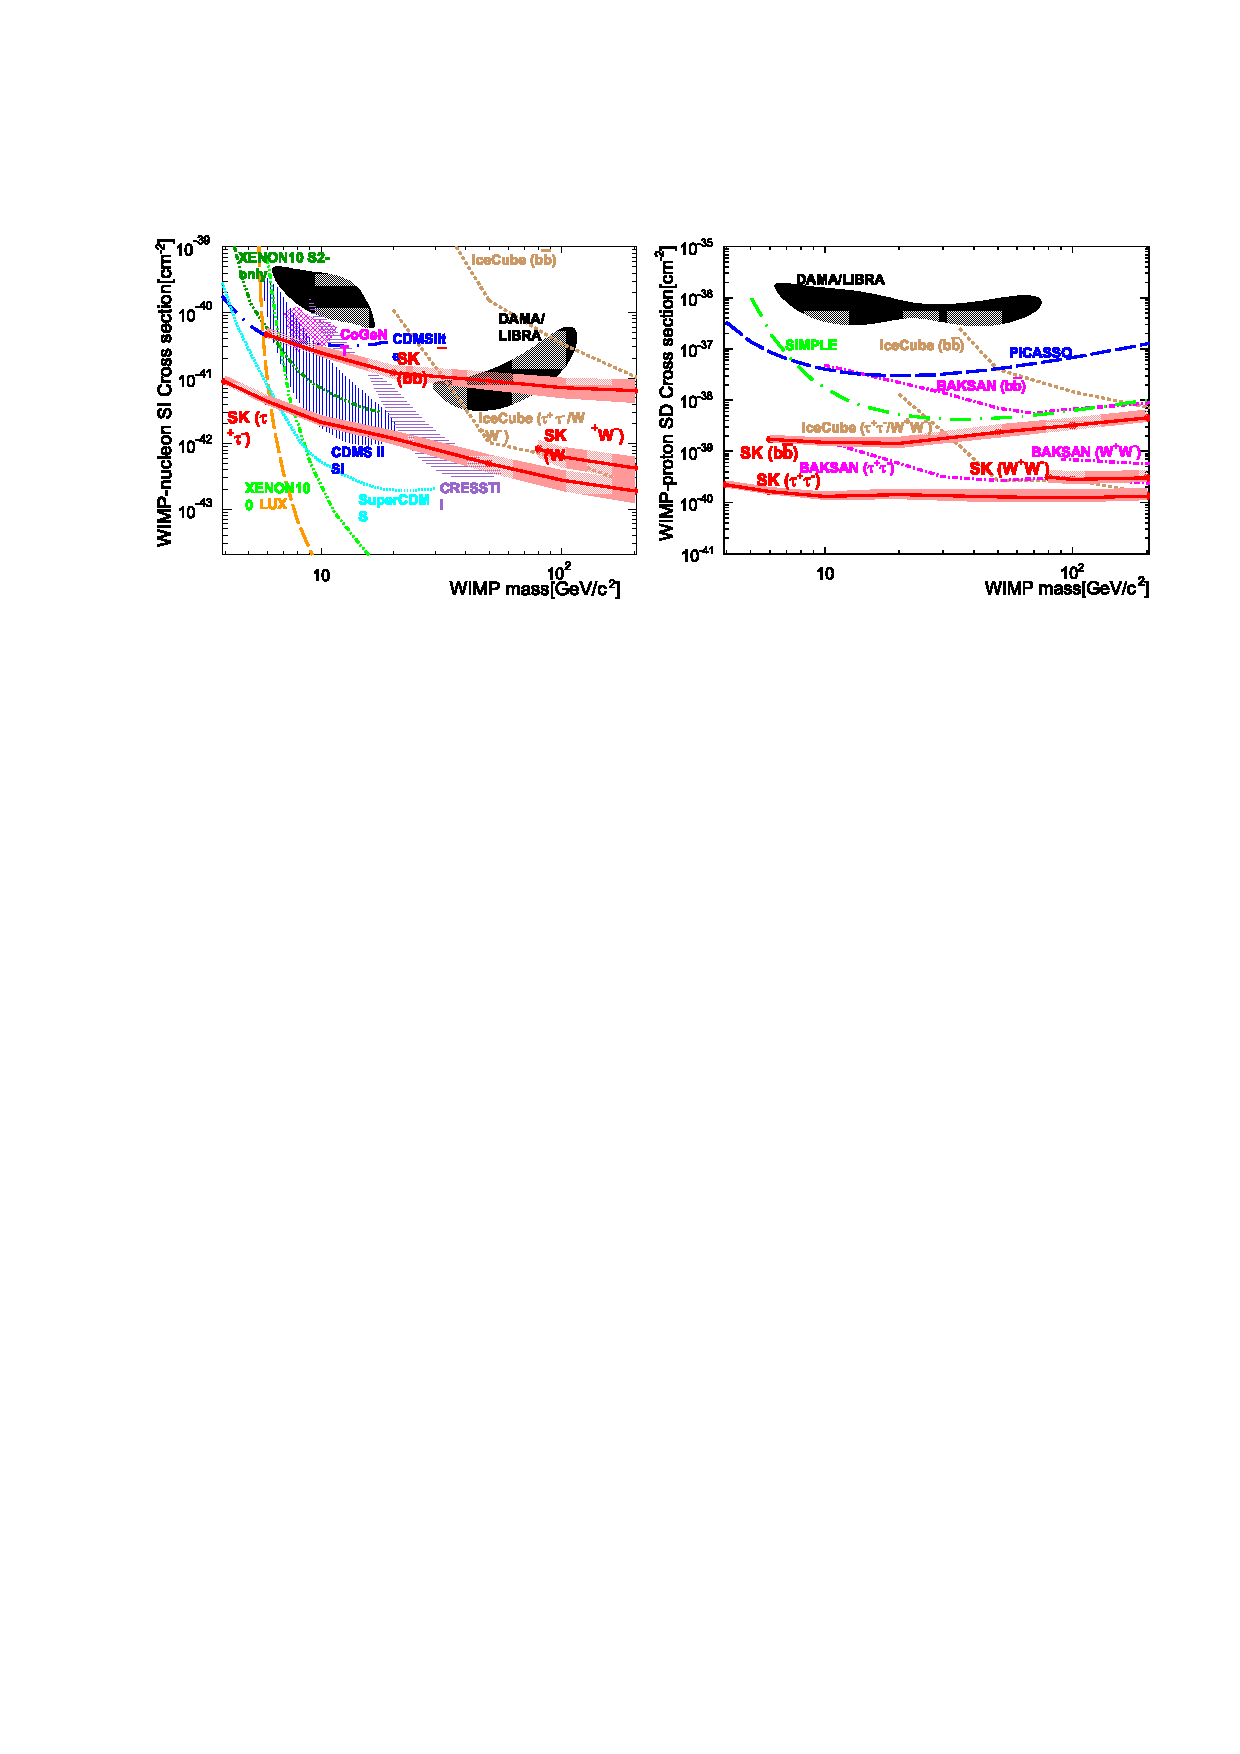
\includegraphics[scale=0.9]{images/SK_graphs.pdf}
		\caption{Ограничения на сечение взаимодействия из разных экспериментов с протоном $\sigma_{\chi p}$. Слева --- для спин независимых взаимодействий, справа для спин зависимых взимодействий \cite{kamiokandecollaboration2015search}.}
	\end{center}
\end{figure}

Поскольку на данный момент ни прямыми, ни косвенными методами не удалось обнаружить частицы темной материи, более сложные модели частиц. Рассматриваемый здесь класс моделей, довольно естественно возникающий во многих теориях, --- это модель двухкомпонентной неупругой темой материи. В таких моделях WIMP имеет основное $\chi$ и возбужденное состояние $\chi^*$ с массами $m_{\chi}$ и $m_{\chi}+\delta$. Изначально такая модификация WIMPов была предложенны для объяснения расхождений между экспериментом DAMA/LIBRA и CDMS \cite{PhysRevD.64.043502}, поскольку от массы мишени зависит, будет ли преодолен энергетический порог $\delta$. Хотя результаты DAMA/LIBRA не смогли воспроизвестись на COSINE-100, такие модели могут ослабить ограничения на сечения, и поэтому представляют интерес.

Важное отличие неупругой темой материи является нетривиальная термализация. Если в упругом случае частицы приходят в больцмановское равновесие, то неупругая ТМ не успевает прийти в термальное равновесие со звездой \cite{Blennow_2018}. Поэтому термализация требует более детального анализа.

Цель данной работы --- получить ограничения на сечения рассеяния частицы темной материи исходя из данных нейтринных обсерваторий, учтя при этом процессы термализации.

